\documentclass[11pt]{article}
\newcommand{\AppName}{linecat}
\newcommand{\AppVersion}{0.14.0}
  % written from pyproject.toml by tools/build_docs.sh
\newcommand{\AppAuthor}{Vahid Anari}
\newcommand{\AppEmail}{vahid.anari8@gmail.com}

\newcommand{\DocName}{User Guide}
\usepackage{style}
\setlength{\emergencystretch}{2em}  % long menu paths in sans serif

% menu paths and keys
\newcommand{\menu}[1]{\textsf{#1}}
\newcommand{\key}[1]{\textsf{#1}}
\newcommand{\then}{\,$\triangleright$\,}

\begin{document}

% ── Title page ────────────────────────────────────────────────────────────────
\begin{titlepage}
  \centering
  \vspace*{3cm}
  {\fontsize{40}{48}\selectfont\bfseries\color{accent} \AppName\par}
  \vspace{0.6cm}
  {\Large Viewer for CDMS spectral line catalogs\par}
  \vspace{2cm}
  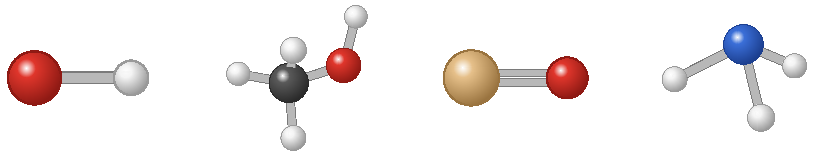
\includegraphics[width=0.8\textwidth]{figures/molecules.pdf}\par
  \vspace{2cm}
  {\Large \DocName\par}
  \vspace{0.3cm}
  {\large Version \AppVersion\par}
  \vfill
  {\large \AppAuthor\par}
  {\small \href{mailto:\AppEmail}{\AppEmail}\par}
  {\small \url{https://github.com/vahid-anari/linecat}\par}
\end{titlepage}

\tableofcontents
\newpage

% ── 1 ─────────────────────────────────────────────────────────────────────────
\section{Getting started}

\AppName{} (Line Catalog Explorer) shows the spectral line catalogs of the Cologne Database for
Molecular Spectroscopy (CDMS) as a table you can filter by quantum numbers and frequency, and
draws the energy levels and transitions of any selection as a diagram that can be saved as PDF
or exported as \LaTeX{} commands.

\subsection{Installing}
\AppName{} needs Python 3.10 or newer. Install it from PyPI with pipx, which gives it an
environment of its own,
\begin{verbatim}
pipx install linecat
\end{verbatim}
or with \texttt{pip install linecat} in an environment of your choice, and start it with
\texttt{linecat}. For development, clone the repository and run \texttt{pip install -e .} in it.

\LaTeX{} is optional: with a \LaTeX{} installation the filter labels and the diagram can be
rendered with real \LaTeX{} (Section~\ref{sec:latex}); without it \AppName{} uses Matplotlib's
built-in math rendering.

\subsection{Starting with a double-click}
Run once
\begin{verbatim}
linecat install-app
\end{verbatim}
This adds \emph{Line Catalog Explorer} with its icon to the Applications folder
(\texttt{\textasciitilde/Applications}, also in Launchpad and Spotlight; drag it to the Dock to keep
it there), to the Start menu on Windows or to the applications menu on Linux. It starts the
\AppName{} of the Python the command was run with, and keeps the \texttt{PATH} of that terminal so
that \LaTeX{} is found as from the terminal. After an update \AppName{} refreshes the launcher by
itself. \texttt{linecat install-app --remove} removes it; run \texttt{linecat install-app} again
if you move or replace that Python.

\subsection{Updating}
A couple of seconds after it starts, \AppName{} asks PyPI in the background whether a newer
version exists; if so it shows what is new (from the release notes) and offers
\menu{Update Now}, which runs \texttt{pipx upgrade linecat} or \texttt{pip install -U linecat},
whichever matches the installation, and then offers a restart. Without an internet connection
nothing is shown. \menu{Help\then Check for Updates\dots} (\key{Cmd+U}) checks on request and also reports when
\AppName{} is up to date. In a terminal, \texttt{linecat update --check} shows whether there is a
newer version, and \texttt{linecat update} installs it (it asks first). A copy installed from a
clone with \texttt{pip install -e} is updated with \texttt{git pull} instead.

\subsection{First start and the built-in catalogs}
\AppName{} ships the CDMS catalog files of four molecules: OH, CH$_3$OH, SiO and NH$_3$. On the
first start, and after every update of \AppName{}, it converts them into CSV catalogs; this takes
about a second. The CSV files are written read-only to the application-data folder
(on macOS \texttt{\textasciitilde/Library/Application Support/linecat/catalogs/}); if one goes
missing it is rebuilt at the next start.

Open one with \menu{File\then Open Built-in Catalog} or with
\key{Cmd+1}--\key{Cmd+4} (OH, CH$_3$OH, SiO, NH$_3$). \menu{File\then Open Built-in
Catalog\then Show Built-in Catalogs Folder} shows the folder in the Finder.

\begin{notebox}
Any other catalog in the same CSV format opens with \menu{File\then Open Catalog\dots}
(\key{Cmd+O}); the last five are listed under \menu{File\then Open Recent}. Section~\ref{sec:convert}
explains how to make such a CSV from a CDMS \texttt{.cat} file.
\end{notebox}

% ── 2 ─────────────────────────────────────────────────────────────────────────
\section{The main window}

\begin{figure}[h]
  \centering
  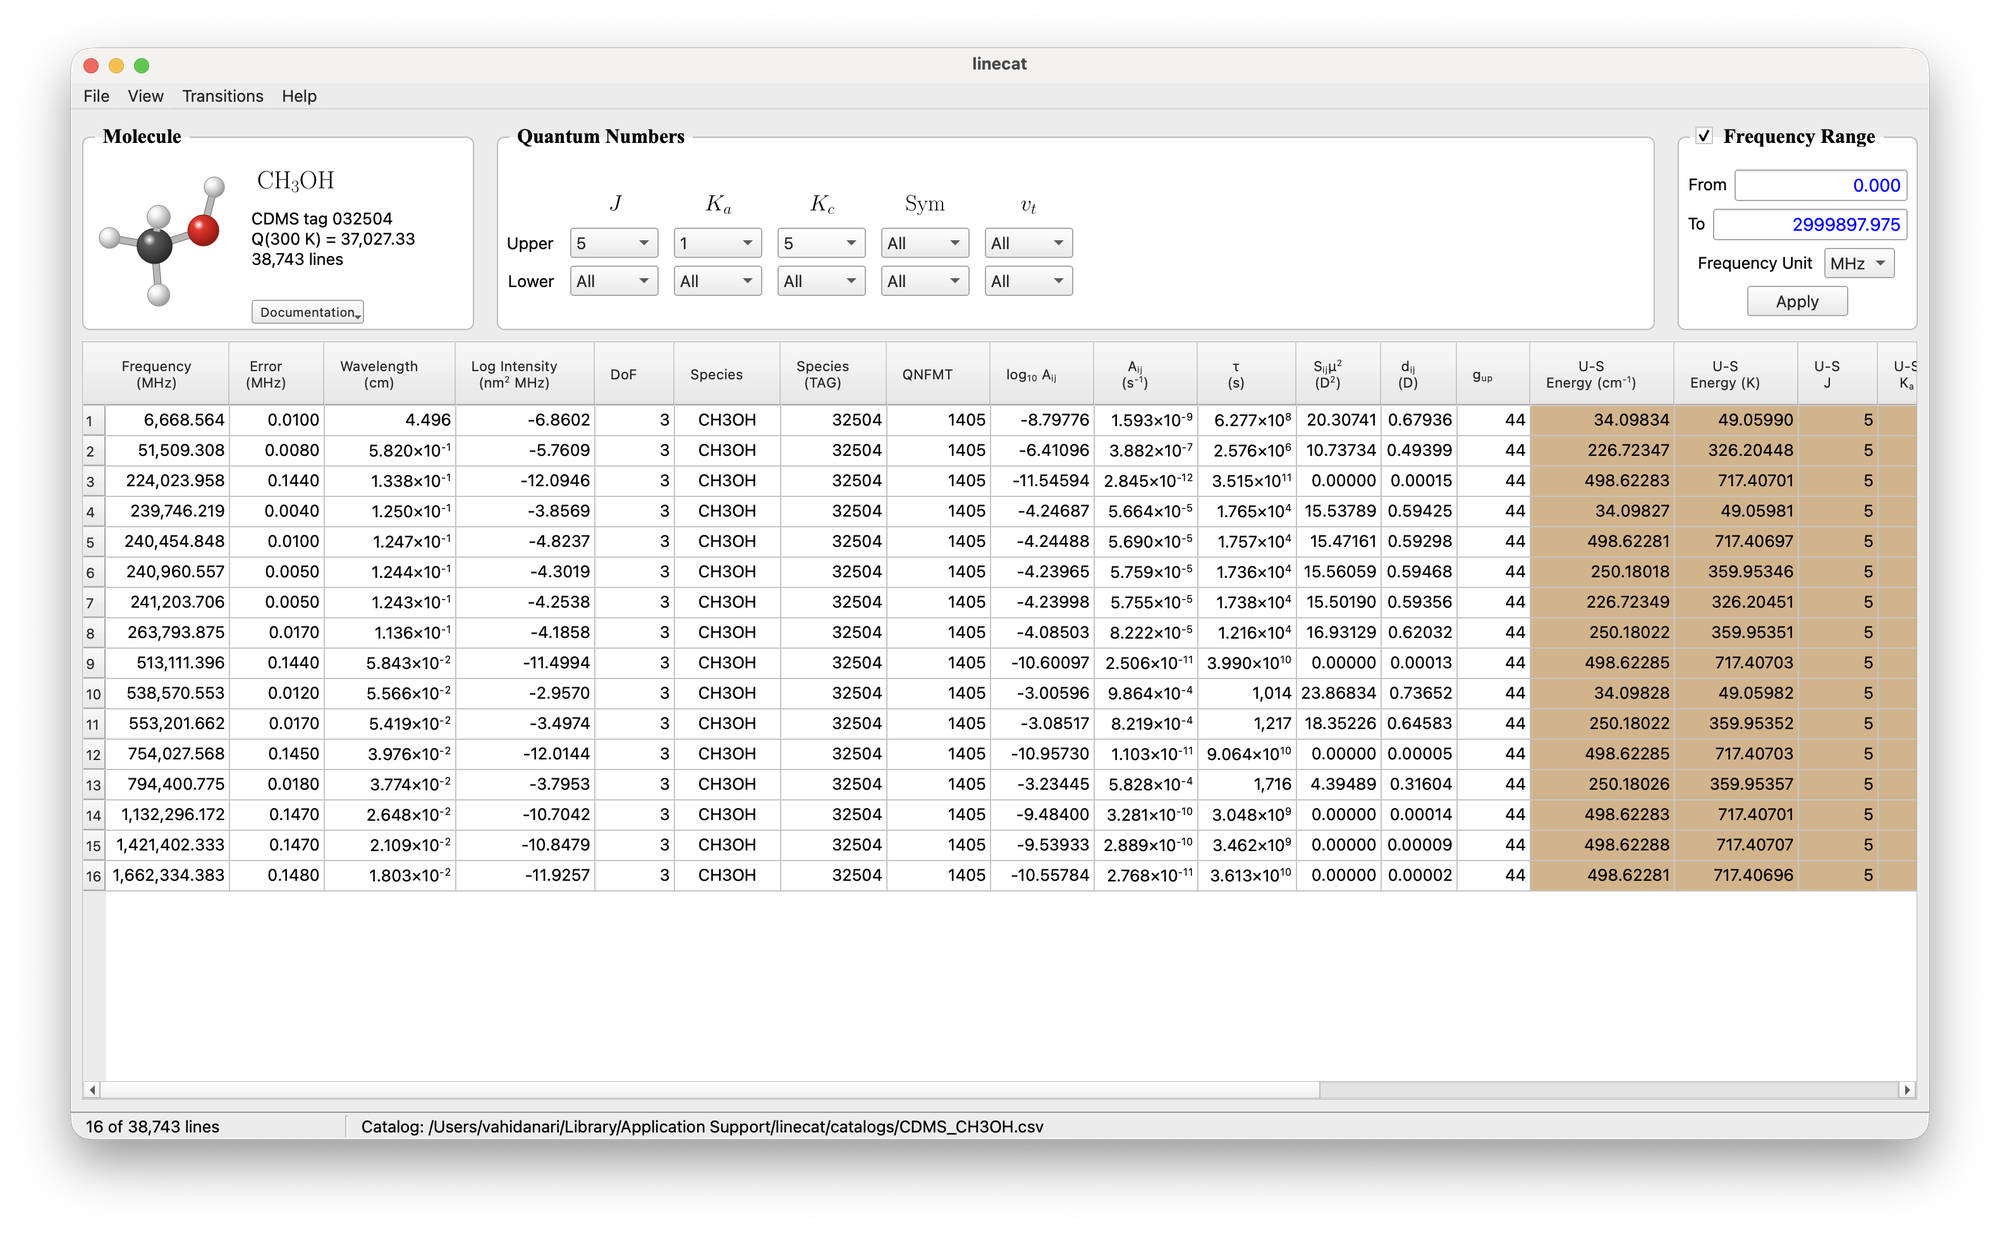
\includegraphics[width=\textwidth]{figures/main_window.png}
  \caption{The main window with the built-in CH$_3$OH catalog, filtered to the transitions from the
    upper level $5_{1,5}$; the first line is the 6.7~GHz methanol maser line.}
  \label{fig:main}
\end{figure}

The top row holds three boxes: the molecule, the quantum-number filters and the frequency range.
Below them is the table of the lines that pass the filters. The status bar shows how many lines
are shown out of how many in the catalog, and the path of the catalog.

\subsection{Molecule}
The \emph{Molecule} box shows a picture of the molecule, its name, the CDMS tag(s) of the catalog
entries, the partition function $Q$ at 300~K used for the line strengths, and the number of lines.
\menu{Documentation} lists the CDMS documentation of the entries (for OH: $v=0$, 1 and 2,
Figure~\ref{fig:molecule}); it is included with \AppName{} and opens without an internet connection.
The general CDMS documents are under \menu{Help\then CDMS Documentation}. The User Guide opens with
\key{Cmd+?}, and \menu{Help\then About Line Catalog Explorer} shows the version, the CDMS credits and the
libraries the app is built on.

\begin{figure}[h]
  \centering
  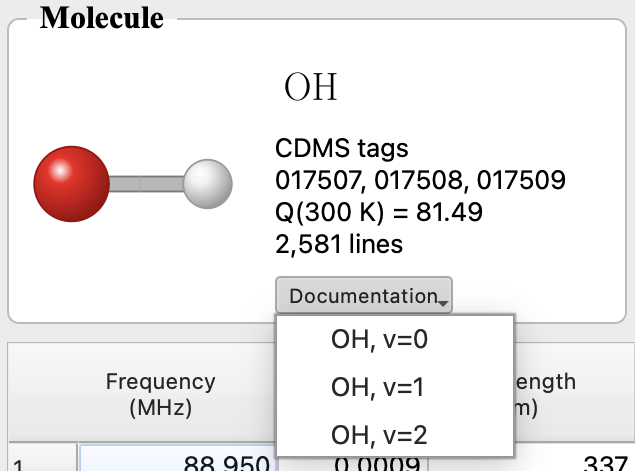
\includegraphics[width=0.45\textwidth]{figures/molecule_docs.png}
  \caption{The Molecule box of the OH catalog with its documentation menu.}
  \label{fig:molecule}
\end{figure}

\subsection{Quantum-number filters}
\emph{Quantum Numbers} has one column per quantum number of the molecule and two rows, for the
upper and the lower state. Each list offers the values that still occur among the lines that pass
the other filters, so the choices narrow as you select. \menu{All} switches a filter off.
\menu{View\then Reset Filters} sets every filter back to \menu{All} and the frequency range back
to the whole catalog.

\subsection{Frequency range}
\emph{From} and \emph{To} set the range in the unit chosen under \emph{Frequency Unit}: Hz, KHz,
MHz, GHz or THz, or a wavelength in \AA, nm, \textmu m, mm or m. \menu{Apply} applies the range.
The check box in the title switches the range off without losing the values typed in.

\subsection{The table}
Click a column header to sort by that column; click again to reverse the order. Right-click a
header for the column menu:
\begin{itemize}[nosep]
  \item \menu{Column Color\dots}, \menu{No Column Color}, \menu{Default Column Color};
  \item \menu{Text Color\dots}, \menu{Default Text Color};
  \item \menu{Alignment} (left, centre, right or the default);
  \item \menu{Hide This Column}, \menu{Choose Columns\dots} (also in \menu{View});
  \item \menu{Reset Colors};
  \item \menu{Font\dots}, \menu{Default Font}.
\end{itemize}
These settings are remembered between sessions. \menu{File\then Export Table as CSV\dots}
(\key{Cmd+E}) writes the filtered lines in the current sort order with all columns, hidden ones
included, so the file opens again in \AppName{} as a catalog of its own.

% ── 3 ─────────────────────────────────────────────────────────────────────────
\section{The energy-level diagram}

\menu{Transitions\then Show Energy-Level Diagram} (\key{Cmd+D}) draws the lines shown in the table
as a diagram of their energy levels and transitions. Above 50 transitions \AppName{} asks before
drawing, since large diagrams take longer to draw; \menu{View\then Large Diagram Warning\dots} in the
main window changes the number or switches the question off.

\begin{figure}[h]
  \centering
  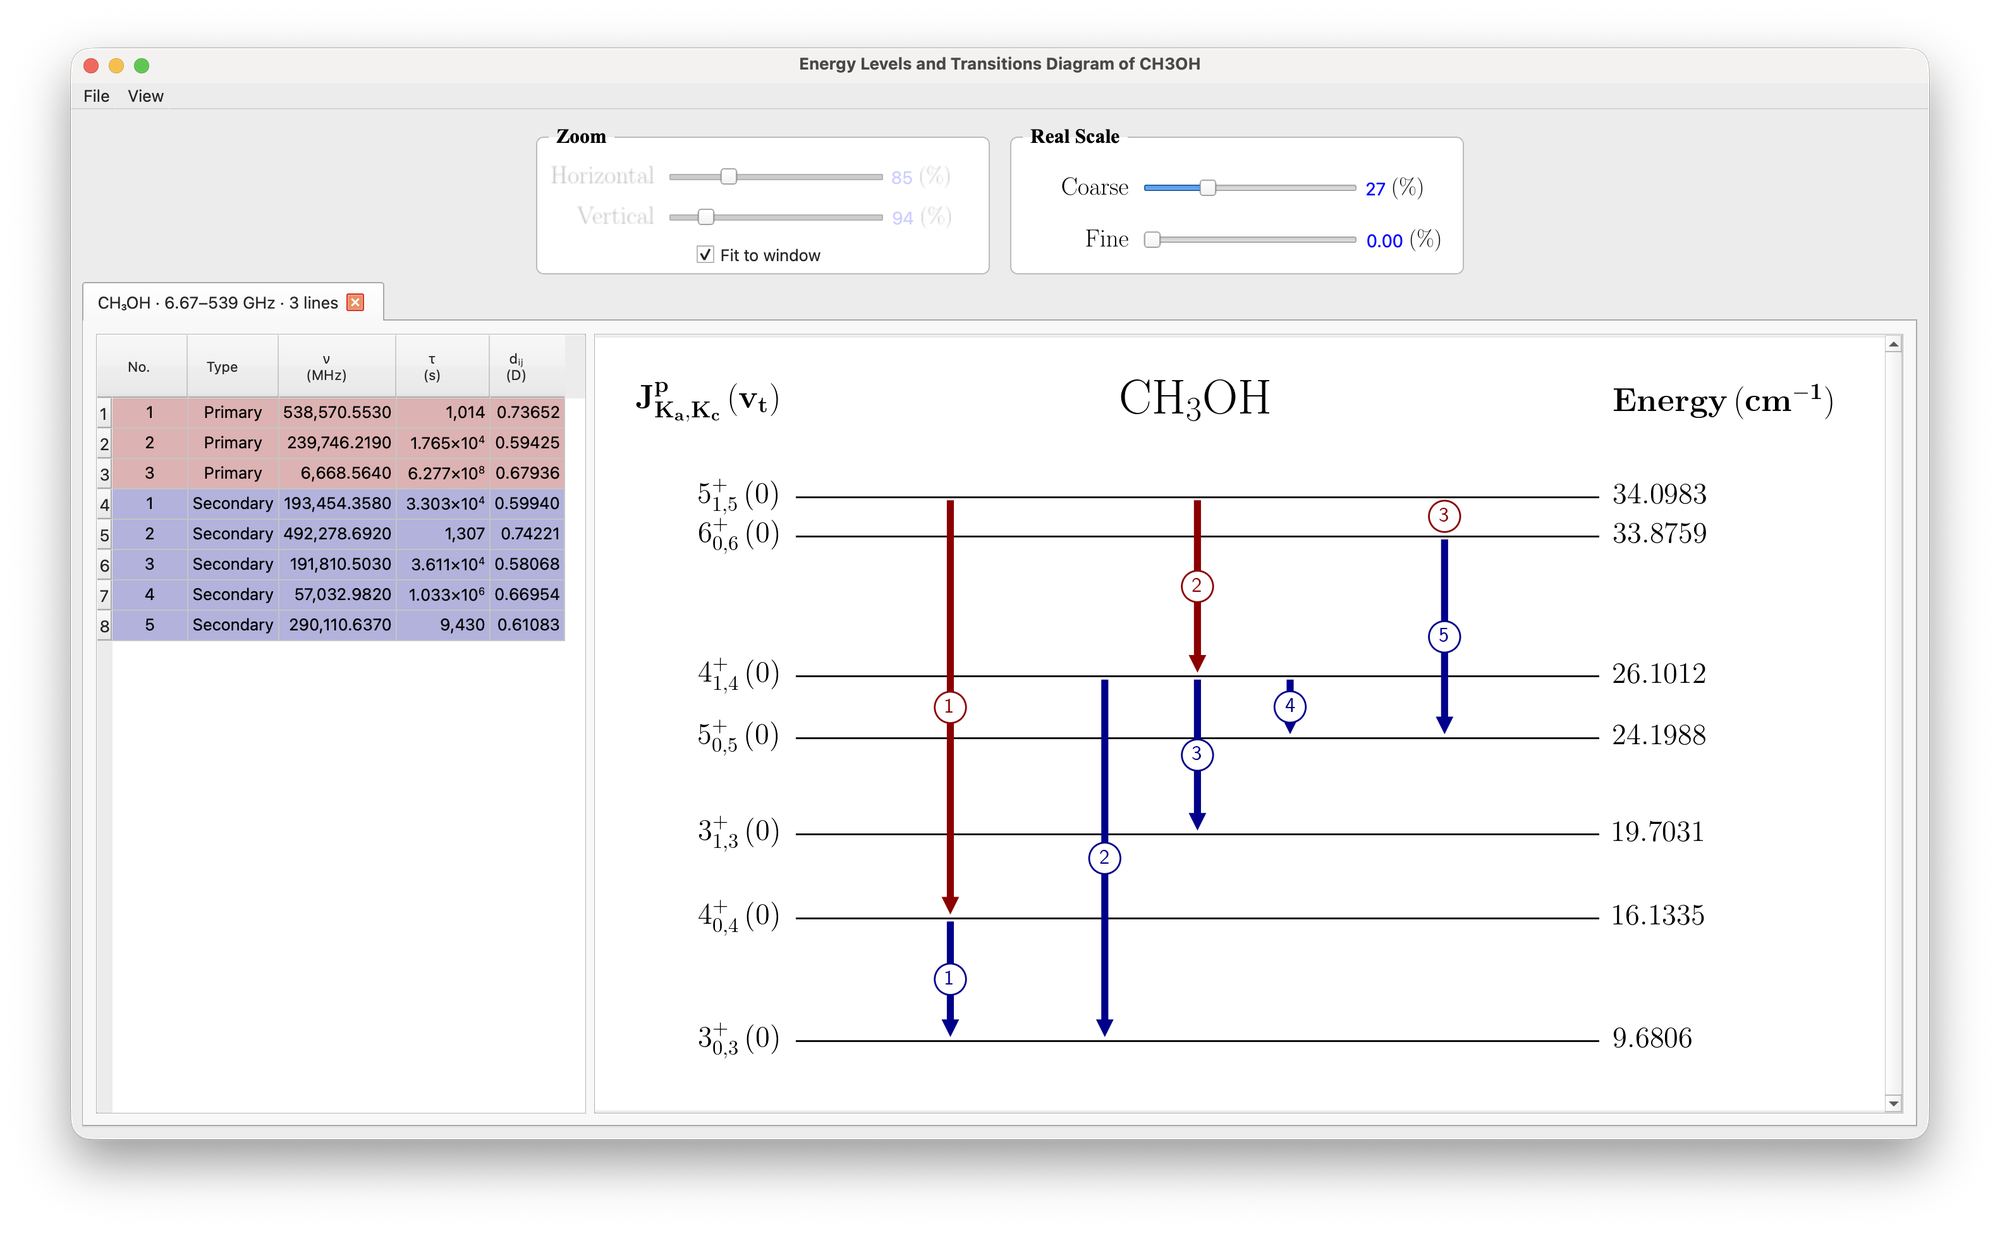
\includegraphics[width=\textwidth]{figures/diagram.png}
  \caption{The diagram window: transition table on the left, diagram on the right. CH$_3$OH,
    three primary transitions (red) with their secondary transitions (blue), drawn with \LaTeX{} at
    27\,\% real scale.}
  \label{fig:diagram}
\end{figure}

\subsection{Levels, transitions and the transition table}
Each level is a horizontal line, labelled with its quantum numbers on the left and its energy
(cm$^{-1}$) on the right; each transition is a numbered arrow from the upper to the lower level.
The table on the left lists the same transitions with their frequency $\nu$, lifetime $\tau$ and
transition dipole moment $d_{ij}$; rows are coloured by type.

The diagram is as large as its content needs: every level gets at least one line of text, and
transitions that would touch are moved apart. Groups of transitions that lie at different heights share
a column, so a large selection grows downwards rather than sideways.

Hovering over an arrow highlights it, its two levels and its row in the table, and shows $\nu$
and $\tau$ next to the pointer, on the side towards the middle of the diagram; hovering over a level highlights the transitions that start or
end on it (Figure~\ref{fig:hover}). The other way round, selecting rows in the table highlights their
arrows.

\begin{figure}[h]
  \centering
  \begin{minipage}{0.495\textwidth}
    \centering
    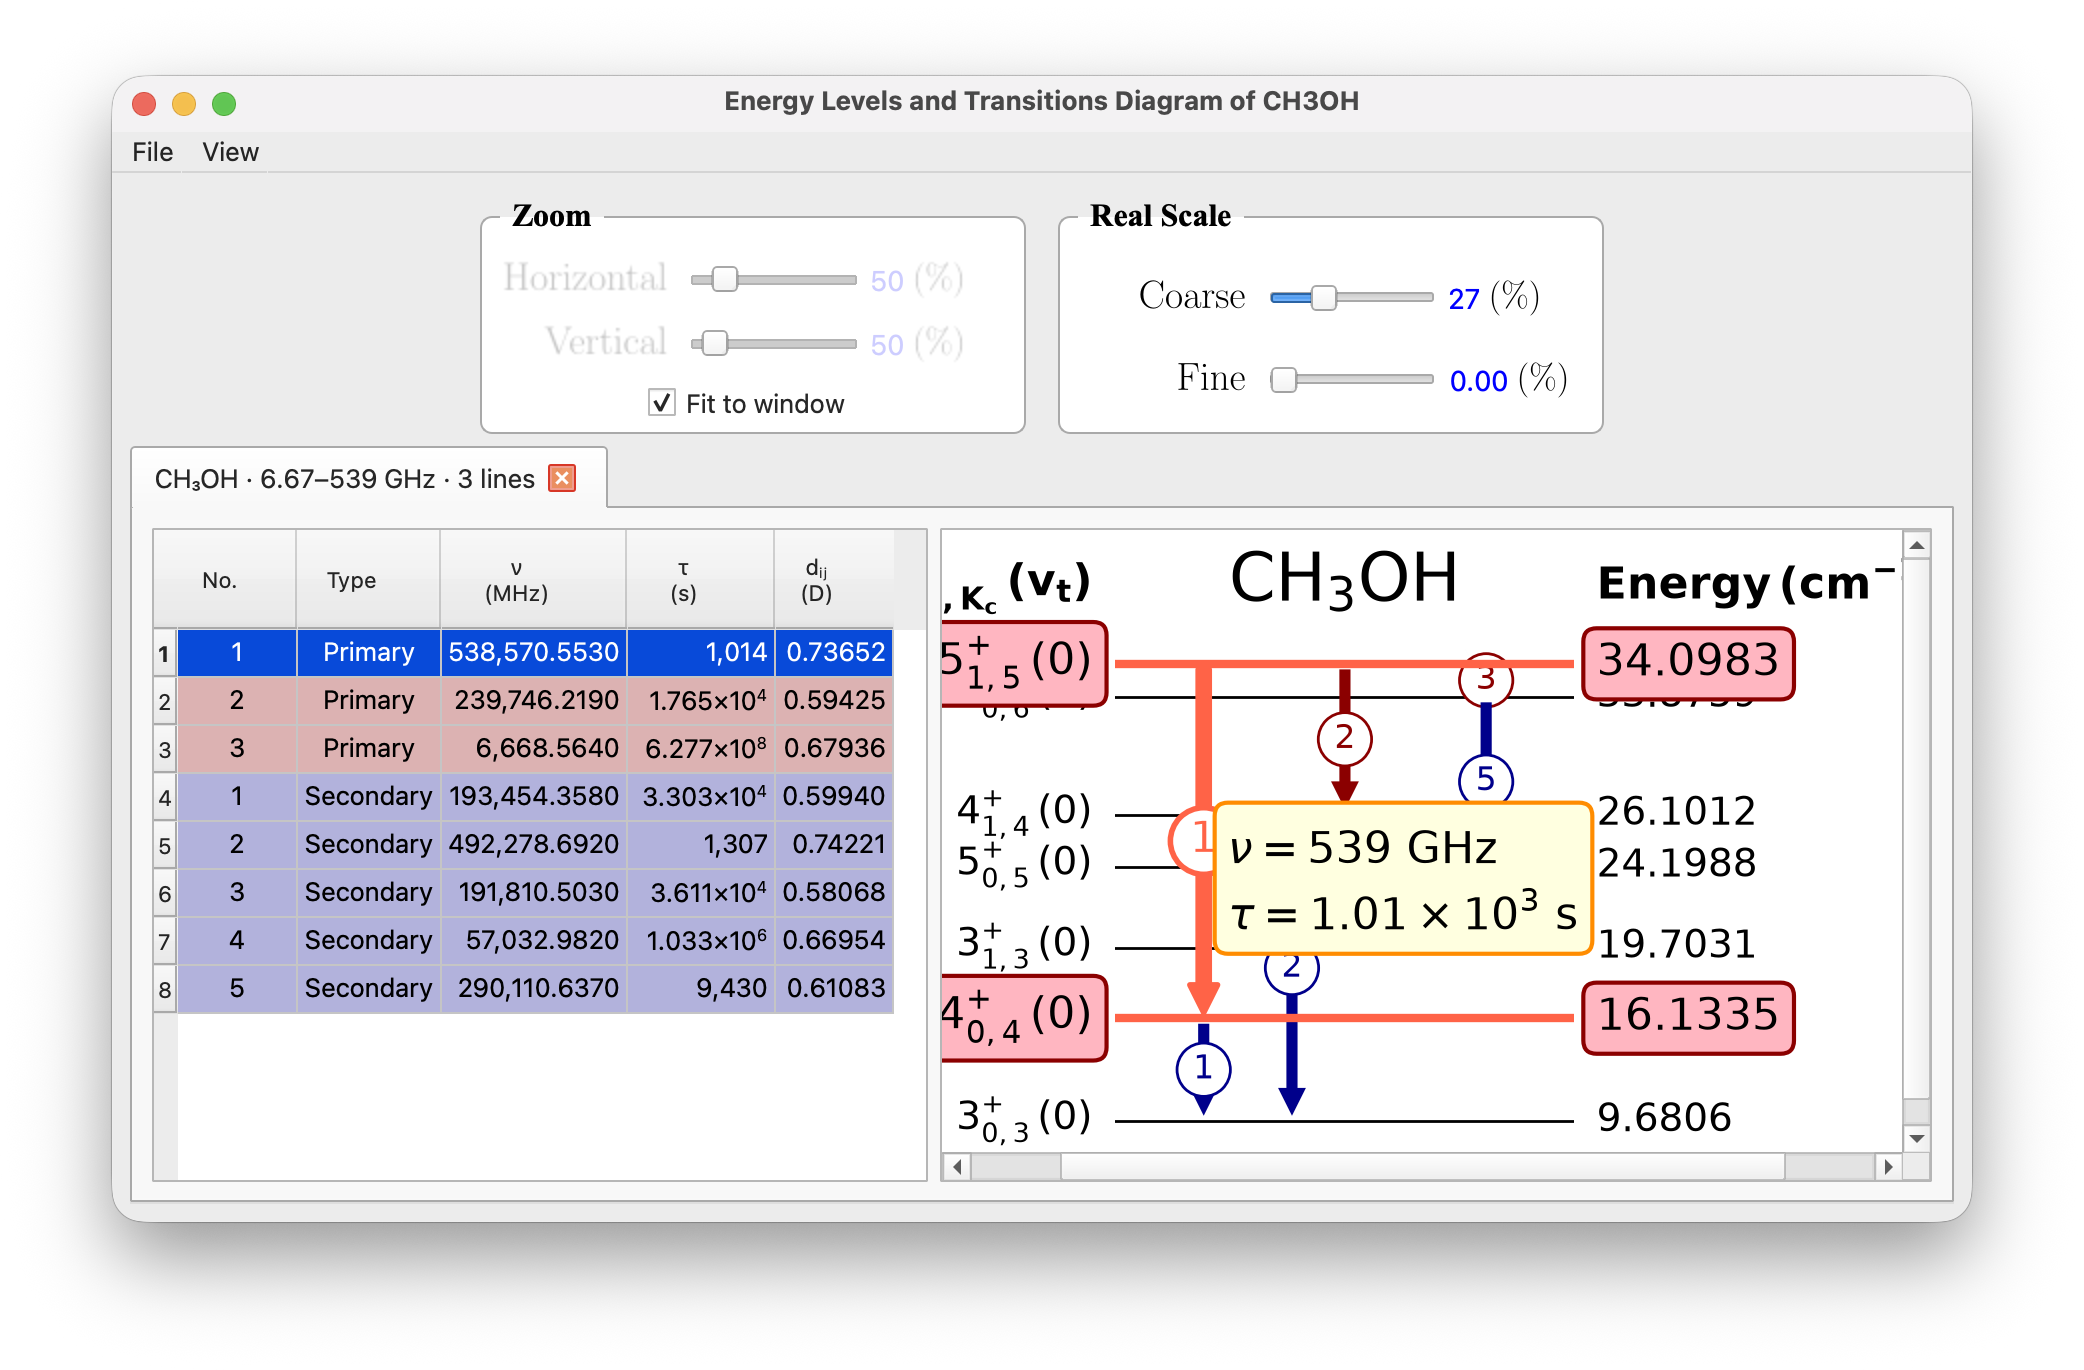
\includegraphics[width=\textwidth]{figures/hover_arrow.png}\\[2pt]
    {\small (a) over an arrow}
  \end{minipage}\hfill
  \begin{minipage}{0.495\textwidth}
    \centering
    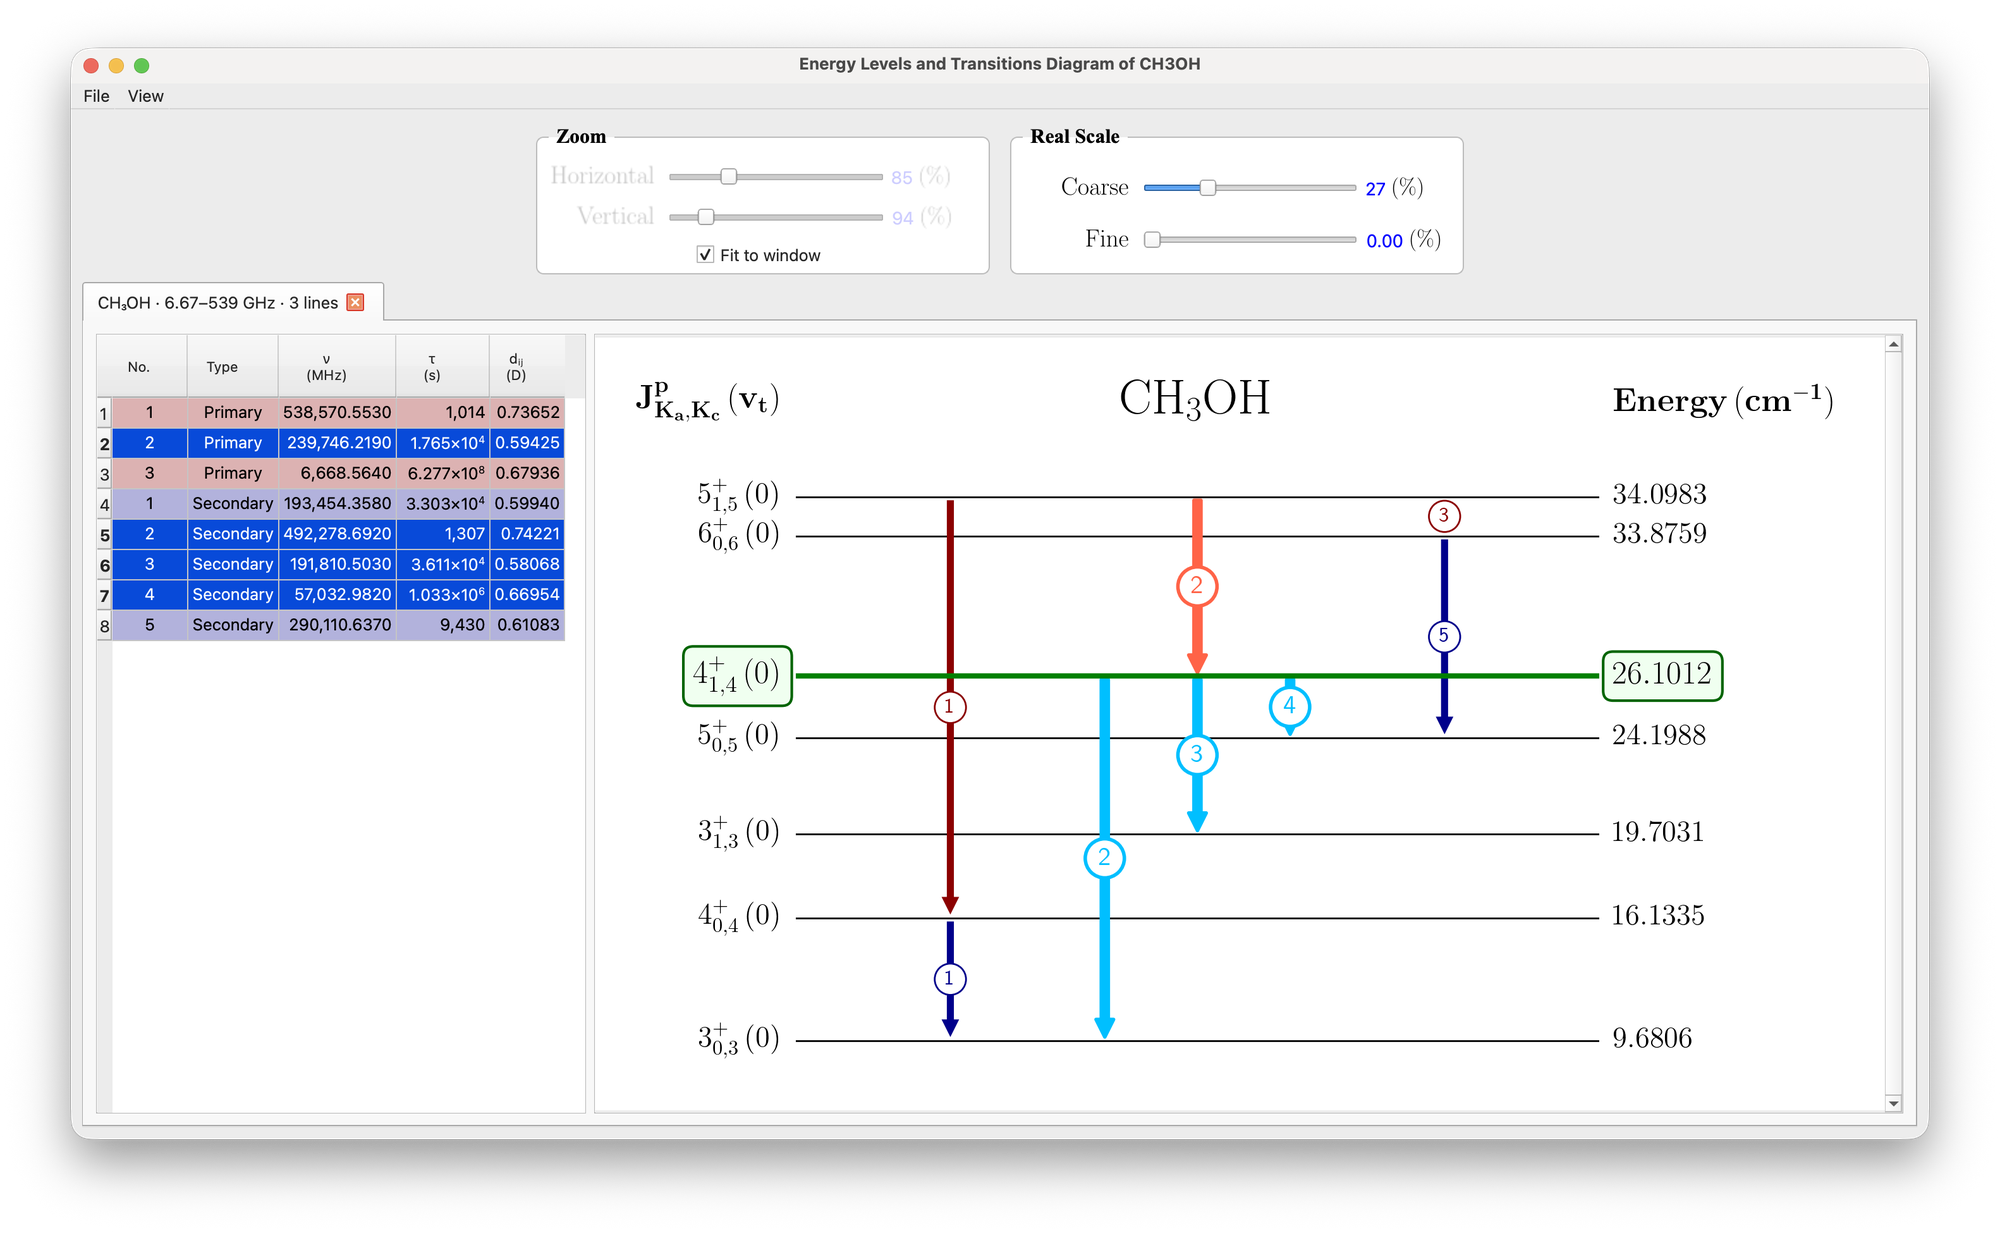
\includegraphics[width=\textwidth]{figures/hover_level.png}\\[2pt]
    {\small (b) over a level}
  \end{minipage}
  \caption{Hovering. (a) The arrow, its two levels and its table row light up, with $\nu$ and $\tau$
    beside the pointer. (b) Every transition that starts or ends on the level lights up, in the
    diagram and in the table.}
  \label{fig:hover}
\end{figure}

\subsection{Tabs and secondary transitions}
The first tab is named after the selection, e.g.\ \emph{NH$_3$ $\cdot$ 18.4--22.2 GHz $\cdot$ 70 lines}.
Double-click an arrow to open a new tab, \emph{From \textrm{(level)}}, with all transitions that start
from its lower level.
\menu{View\then Secondary Transitions} adds to the current tab the transitions that leave the
lower levels of the primary ones (drawn in blue). Each tab keeps its own settings; the first tab cannot be closed.

\subsection{Zoom and real scale}
\menu{Fit to window} (check box under the zoom sliders, or \menu{View\then Fit to Window},
\key{Cmd+0}) scales the diagram to the space beside the table and follows the window when it is
resized, but never below the size at which the labels stay apart: a larger diagram scrolls instead.
Switch it off to set the \emph{Horizontal} and \emph{Vertical} zoom by hand.

On a trackpad, pinch to zoom in and out around the point between your fingers, as in a PDF viewer;
with a mouse, turn the wheel while holding \key{Cmd}. Both switch \menu{Fit to window} off and move the
zoom sliders along; a two-finger double tap switches it on again. Two fingers dragging, or the wheel,
scroll the diagram as before.

By default the levels are evenly spaced, in order of energy. The \emph{Real Scale} sliders move
them towards their true energies: \emph{Coarse} (0--95\,\%) and \emph{Fine} (0--5\,\%) add up to
the fraction of the true spacing used, 100\,\% being energies to scale.

\subsection{\LaTeX{} rendering}\label{sec:latex}
\menu{View\then Use LaTeX for Rendering} redraws the diagram with \LaTeX{}. The labels are
rendered in the background behind a progress dialog the first time; \LaTeX{} keeps the results,
so later drawings are quick. In the main window, \menu{View\then Use LaTeX for Labels} does the
same for the filter labels.

\subsection{Saving}
\menu{File\then Save Figure as PDF\dots} (\key{Cmd+S}) writes a two-page PDF: the diagram, then the
transition table.

\menu{File\then LaTeX Commands\dots} lists the levels and transitions of the tab as two \LaTeX{}
commands, for drawing your own diagram; \menu{Copy} puts them on the clipboard and \menu{Save\dots}
writes a \texttt{.tex} file. For the diagram of Figure~\ref{fig:diagram}:
\begin{verbatim}
% CH3OH · 6.67-539 GHz · 3 lines -- linecat 0.10.3
\Level{L1}{$3_{0, 3}^{+}\,(0)$}{9.6806}
...
\Level{L7}{$5_{1, 5}^{+}\,(0)$}{34.0983}
\Transition{pri}{1}{L7}{L2}{538570.553}{1.014e3}
...
\Transition{sec}{1}{L2}{L1}{193454.358}{3.303e4}
\end{verbatim}
\begin{tabular}{@{}>{\ttfamily}l l@{}}
  \toprule
  \textrm{Command} & Arguments\\
  \midrule
  \textbackslash Level & name, label (as in the diagram), energy in cm$^{-1}$\\
  \textbackslash Transition & type (\texttt{pri} or \texttt{sec}), number, upper and lower level,\\
                            & frequency in MHz, lifetime in s\\
  \bottomrule
\end{tabular}

Levels are named \texttt{L1}, \texttt{L2}, \dots{} from the lowest energy up, so the transitions refer
to them by name; numbers are the catalog's. \AppName{} does not define the two commands: write them as
you like, for instance with TikZ, storing each level's position under its name with
\verb|\coordinate| and drawing an arrow between two names; \verb|\num| from \texttt{siunitx} prints
the numbers. A level that the catalog lists only as an upper state gets the energy of its first line
(lower energy $+\,h\nu$); the others get the lower-state energy as listed by CDMS.

% ── 4 ─────────────────────────────────────────────────────────────────────────
\section{Converting CDMS catalogs}\label{sec:convert}

The built-in catalogs cover OH, CH$_3$OH, SiO and NH$_3$. To use a newer CDMS release, download
the \texttt{.cat} files of the entries from \url{https://cdms.astro.uni-koeln.de/} and put them in a
folder per species, named as in \AppName{} (\texttt{OH/c017507.cat}, \dots). Then choose
\menu{File\then Convert CDMS Catalogs\dots} and select either the folder that holds the species
folders or a single species folder. The CSV files are written next to the \texttt{.cat} files; a
progress dialog and a short report follow. A single converted catalog opens by itself.

For each line the converter computes the wavelength, the upper-state energy, both energies in
kelvin, the Einstein coefficient $A_{ij}$, the lifetime $\tau = 1/A_{ij}$, the line strength
$S_{ij}\mu^2$ and the transition dipole moment $d_{ij}$, using the relations in
Appendix~\ref{app:equations}.

% ── 5 ─────────────────────────────────────────────────────────────────────────
\section{Command line}

\begin{tabular}{@{}>{\ttfamily}l l@{}}
  \toprule
  linecat & open the viewer\\
  linecat CATALOG.csv & open a catalog at start\\
  linecat convert & convert the built-in CDMS files (into the current folder)\\
  linecat convert OH SiO & convert some species\\
  linecat convert --catalogs DIR & convert your own \texttt{.cat} files in DIR\\
  \dots{} --output-dir OUT & write the CSV files to OUT\\
  linecat update & update from PyPI (asks first)\\
  linecat update --check & only show whether a newer version exists\\
  linecat install-app & add the app to Applications / the Start menu\\
  linecat install-app --remove & remove it again\\
  linecat --version & show the version\\
  \bottomrule
\end{tabular}

% ── 6 ─────────────────────────────────────────────────────────────────────────
\section{Adding a species}

A species is described in \texttt{linecat/molecules.py} by a \texttt{MoleculeInfo}: its name, the
\texttt{.cat} files, the partition function and temperature, the quantum numbers of the CDMS
format and the filters shown in the window. Two functions complete it:
\texttt{<name>\_standardize(df, prefix)}, which turns the raw quantum numbers into the ones shown
(for example $\Omega$ and the parity of OH), working on whole columns of the table, and
\texttt{<name>\_label(df, prefix)}, which writes the level labels of the diagram. Register the
species in \texttt{REGISTRY} and put its \texttt{.cat} files, the CDMS documentation PDFs of its
entries and a picture \texttt{<SPECIES>.svg} in \texttt{linecat/data/molecules/<SPECIES>/}.

% ── References ────────────────────────────────────────────────────────────────
\section*{References}
\addcontentsline{toc}{section}{References}
The catalog data come from the Cologne Database for Molecular Spectroscopy; please cite
\begin{itemize}[nosep]
  \item H.\,S.\,P. Müller et al., 2001, Astron. Astrophys. 370, L49;
  \item H.\,S.\,P. Müller et al., 2005, J. Mol. Struct. 742, 215;
  \item C.\,P. Endres et al., 2016, J. Mol. Spectrosc. 327, 95.
\end{itemize}
The catalog format and the SPCAT program are described by H.\,M. Pickett et al., 1998,
J. Quant. Spectrosc. Radiat. Transfer 60, 883. The CDMS documentation pages included with
\AppName{} are reproduced with credit to CDMS.

% ── Appendix ──────────────────────────────────────────────────────────────────
\newpage
\appendix
% Equations behind the A_ij, d_ij, S_ij and energy columns (Vahid Anari, "Some useful equations").
% Included as an appendix of the User Guide.
\providecommand{\unit}[1]{\,\mathrm{#1}}
\providecommand{\inunit}[2]{\left[\frac{#1}{\mathrm{#2}}\right]}
\providecommand{\bz}[1]{e^{-#1/kT}}

\section{Equations}\label{app:equations}
These are the relations \texttt{linecat convert} uses to derive the radiative quantities of each line
from the CDMS catalog entries (frequency, intensity at $T=300$~K, lower-state energy, upper-state
degeneracy and the partition function $Q_{rs}(300\,\mathrm{K})$).
\textcolor{warnborder}{All equations are in cgs units.}

\subsection{Constants and conversion factors}
\begin{equation}
\begin{aligned}
  h   &= 6.62607015\times10^{-27}\unit{erg\cdot s}\\
  k_B &= 1.380649\times10^{-16}\unit{erg\cdot K^{-1}}\\
  c   &= 2.99792458\times10^{10}\unit{cm\cdot s^{-1}}\\
  1\unit{D} &= 10^{-18}\unit{statC\cdot cm}\\
  1\unit{erg} &= \mathrm{statC^2\cdot cm^{-1}}\\
  {}^{x}S_{ij}\,\mu_x^2 &= g_i\,\mu_{ij}^2
\end{aligned}
\end{equation}

\subsection{Conversion relations (Section~\ref{app:a})}
Frequency ($\mathrm{MHz}\to\mathrm{cm^{-1}}$):
\begin{equation}
  \inunit{\tilde\nu}{cm^{-1}} = 3.33564095\times10^{-5}\inunit{\nu}{MHz}
\end{equation}
Energy ($\mathrm{cm^{-1}}\to\mathrm{K}$):
\begin{equation}
  \inunit{T}{K} = 1.43877688\inunit{\tilde\nu}{cm^{-1}}
\end{equation}

\subsection{Intensity}
The intensity $I(T)$ is calculated according to
\begin{equation}
  I(T) = \frac{8\pi^3}{3hc}\,\nu\,S_g\,\mu_g^2\,
         \frac{\bz{E''}-\bz{E'}}{Q_{rs}(T)}
\end{equation}
with $\nu$ and $S_g$ the line frequency and strength, $\mu_g$ the dipole moment along the
molecular $g$-axis, $E''$ and $E'$ the lower and upper state energy, and $Q_{rs}$ the
rotation-spin partition function at the temperature~$T$.
With $I(T)$ in $\mathrm{nm^2\,MHz}$, $\nu$ in MHz and $\mu_g$ in D one obtains
(Section~\ref{app:b})
\begin{equation}
  I(T) = \nu\,S_g\,\mu_g^2\,\frac{\bz{E''}-\bz{E'}}{Q_{rs}(T)}\;
         4.16237896\times10^{-5}\unit{nm^2\,MHz}
\end{equation}

\subsection{Spontaneous emission rate}
The average spontaneous emission rate from the upper states into the lower states is
\begin{equation}
  A = \frac{8\pi\nu^2}{c^2}\,I(T)\left(\frac{Q_{rs}(T)}{g_{up}}\right)
      \left[\bz{E''}-\bz{E'}\right]^{-1}
\end{equation}
in which $g_{up}$ is the degeneracy of the upper state.
With $I(T)$ in $\mathrm{nm^2\,MHz}$ and $\nu$ in MHz one obtains (Section~\ref{app:b})
\begin{equation}
  A = I(T)\,\nu^2\left[Q_{rs}(T)/g_{up}\right]
      \left[\bz{E''}-\bz{E'}\right]^{-1}\,2.79639459\times10^{-16}\unit{s^{-1}}
\end{equation}

\noindent\textcolor{red}{Note:} numerical problems may occur in this equation if the
frequency $\nu$ is small with respect to the lower state energy $E''$. So, if
$\bz{E''}-\bz{E'}=0$ numerically, we use
\begin{equation}
  \bz{E''}-\bz{E'} \simeq \frac{h\nu}{kT}\,\bz{E''}
\end{equation}

\subsection{Transition dipole moment}
\begin{equation}
  \mu^2 = \frac{3hc^3}{64\pi^4\nu^3}\,A
\end{equation}
With $A$ in $\mathrm{s^{-1}}$ and $\nu$ in MHz one obtains (Section~\ref{app:b})
\begin{equation}
  \mu = \sqrt{\frac{A}{\nu^3}}\;9.26894\times10^{9}\unit{D}
\end{equation}

\subsection{Derivation of the conversion relations}\label{app:a}
\begin{align*}
  \inunit{\tilde\nu}{cm^{-1}} &= \frac1c\inunit{\nu}{Hz}
                               = 3.33564095\times10^{-5}\inunit{\nu}{MHz}\\[4pt]
  \inunit{\tilde\nu}{cm^{-1}} &= \frac1{hc}\inunit{E}{erg}
                               = 5.03411657\times10^{15}\inunit{E}{erg}\\[4pt]
  \inunit{T}{K} &= \frac1{k_B}\inunit{E}{erg}
                 = \frac{hc}{k_B}\inunit{\tilde\nu}{cm^{-1}}
                 = 1.43877688\inunit{\tilde\nu}{cm^{-1}}
\end{align*}

\subsection{Derivation of the radiative quantities}\label{app:b}
Here $i$ is the upper and $j$ the lower state.

\subsubsection*{Intensity}
\begin{align*}
  I_{ij}(T) &= \frac{8\pi^3}{3hc}\,\nu_{ij}\,{}^{x}S_{ij}\mu_x^2\,
               \frac{\bz{E_j}-\bz{E_i}}{Q_{rs}(T)}\\
  &= 4.16237896\times10^{17}
     \left(\frac{\nu_{ij}}{\mathrm{Hz}}\right)
     \left(\frac{{}^{x}S_{ij}\mu_x^2}{\mathrm{statC^2\cdot cm^2}}\right)
     \frac{\bz{E_j}-\bz{E_i}}{Q_{rs}(T)}\;
     \frac{\mathrm{Hz\cdot statC^2\cdot cm^2}}{\mathrm{erg\cdot s\cdot cm\cdot s^{-1}}}\\
  &= 4.16237896\times10^{17}
     \left(\frac{\nu_{ij}}{\mathrm{Hz}}\right)
     \left(\frac{{}^{x}S_{ij}\mu_x^2}{\mathrm{statC^2\cdot cm^2}}\right)
     \frac{\bz{E_j}-\bz{E_i}}{Q_{rs}(T)}\unit{cm^2\,Hz}\\
  &= 4.16237896\times10^{31}
     \left(\frac{\nu_{ij}}{\mathrm{MHz}}\right)
     \left(\frac{{}^{x}S_{ij}\mu_x^2}{\mathrm{statC^2\cdot cm^2}}\right)
     \frac{\bz{E_j}-\bz{E_i}}{Q_{rs}(T)}\unit{nm^2\,MHz}\\
  &= 4.16237896\times10^{31}
     \left(\frac{\nu_{ij}}{\mathrm{MHz}}\right)
     \left(\frac{{}^{x}S_{ij}\mu_x^2}{\mathrm{D^2}}\,
           \frac{\mathrm{D^2}}{\mathrm{statC^2\cdot cm^2}}\right)
     \frac{\bz{E_j}-\bz{E_i}}{Q_{rs}(T)}\unit{nm^2\,MHz}\\
  &= 4.16237896\times10^{-5}
     \left(\frac{\nu_{ij}}{\mathrm{MHz}}\right)
     \left(\frac{{}^{x}S_{ij}\mu_x^2}{\mathrm{D^2}}\right)
     \frac{\bz{E_j}-\bz{E_i}}{Q_{rs}(T)}\unit{nm^2\,MHz}
\end{align*}
\begin{equation*}
  \inunit{I_{ij}(T)}{nm^2\,MHz} = 4.16237896\times10^{-5}
     \left(\frac{\nu_{ij}}{\mathrm{MHz}}\right)
     \left(\frac{{}^{x}S_{ij}\mu_x^2}{\mathrm{D^2}}\right)
     \frac{\bz{E_j}-\bz{E_i}}{Q_{rs}(T)}
\end{equation*}

\subsubsection*{Einstein A coefficient}
\begin{align*}
  A_{ij} &= \frac{64\pi^4\nu_{ij}^3}{3hc^3}\,\mu_{ij}^2
          = \frac{64\pi^4\nu_{ij}^3}{3hc^3}\,\frac{{}^{x}S_{ij}\mu_x^2}{g_i}\\
  &= \frac{64\pi^4\nu_{ij}^3}{3hc^3}\,\frac1{g_i}
     \left\{\frac{I_{ij}(T)\,Q_{rs}(T)}
                 {\frac{8\pi^3}{3hc}\,\nu_{ij}\left[\bz{E_j}-\bz{E_i}\right]}\right\}
   = \frac{8\pi\nu_{ij}^2}{c^2}\,\frac{I_{ij}(T)\,Q_{rs}(T)}{g_i}
     \left[\bz{E_j}-\bz{E_i}\right]^{-1}\\
  &= 2.79639459\times10^{-20}\inunit{I_{ij}(T)}{nm^2\,MHz}\inunit{\nu_{ij}}{Hz}^{2}
     \left[Q_{rs}(T)/g_i\right]\left[\bz{E_j}-\bz{E_i}\right]^{-1}
     \frac{\mathrm{nm^2\,MHz\cdot Hz^2}}{\mathrm{cm^2\,s^{-2}}}\\
  &= \inunit{I_{ij}(T)}{nm^2\,MHz}\inunit{\nu_{ij}}{MHz}^{2}
     \left[Q_{rs}(T)/g_i\right]\left[\bz{E_j}-\bz{E_i}\right]^{-1}
     2.79639459\times10^{-16}\unit{s^{-1}}
\end{align*}
\begin{equation*}
  \inunit{A_{ij}}{s^{-1}} = 2.79639459\times10^{-16}\inunit{I_{ij}(T)}{nm^2\,MHz}
     \inunit{\nu_{ij}}{MHz}^{2}\left[Q_{rs}(T)/g_i\right]e^{E_j/kT}
     \left[1-e^{-h\nu_{ij}/kT}\right]^{-1}
\end{equation*}

\noindent\textcolor{red}{Note:} if $\bz{E''}-\bz{E'}=0$ numerically, we use
\begin{equation*}
  \bz{E''}-\bz{E'} = \bz{E''}\left(1-e^{-(E'-E'')/kT}\right)
                   = \bz{E''}\left(1-e^{-h\nu/kT}\right)
                   \simeq \frac{h\nu}{kT}\,\bz{E''}
\end{equation*}

\subsubsection*{Transition dipole moment}
\begin{align*}
  \mu_{ij}^2 &= \frac{3hc^3}{64\pi^4\nu_{ij}^3}\,A_{ij}\\
  &= 85.9132065\inunit{A_{ij}}{s^{-1}}\inunit{\nu_{ij}}{Hz}^{-3}
     \frac{\mathrm{erg\cdot s\cdot cm^3\cdot s^{-3}}}{\mathrm{s\cdot Hz^3}}
   = 85.9132065\inunit{A_{ij}}{s^{-1}}\inunit{\nu_{ij}}{Hz}^{-3}\unit{statC^2\cdot cm^2}\\
  &= 8.59132065\times10^{19}\inunit{A_{ij}}{s^{-1}}\inunit{\nu_{ij}}{MHz}^{-3}\unit{D^2}
\end{align*}
\begin{equation*}
  \inunit{\mu_{ij}}{D} = \sqrt{8.59132065\times10^{19}\inunit{A_{ij}}{s^{-1}}
                                \inunit{\nu_{ij}}{MHz}^{-3}}
\end{equation*}



\end{document}
